\documentclass[letterpaper]{article}
\usepackage{natbib,alifexi}
\usepackage[english]{babel}
\usepackage{blindtext}
\usepackage{xcolor}
\usepackage{microtype}
\usepackage{amsmath}
\usepackage{listings}
\usepackage{capt-of}
\usepackage{float}

\definecolor{dkgreen}{rgb}{0,0.6,0}
\definecolor{gray}{rgb}{0.5,0.5,0.5}
\definecolor{mauve}{rgb}{0.58,0,0.82}

\lstset{frame=none,
 language=Scala,
 aboveskip=3mm,
 belowskip=3mm,
 showstringspaces=false,
 columns=flexible,
 xleftmargin=.25in,
 basicstyle={\footnotesize \ttfamily},
 numbers=left,
 numberstyle=\tiny \color{black},
 keywordstyle=\color{blue},
 commentstyle=\color{dkgreen},
 stringstyle=\color{mauve},
 breaklines=true,
 breakatwhitespace=true,
 tabsize=3
}

\newcommand\todo[1]{\textcolor{orange}{Todo: #1}}

\title{Review: Accelerating Multi-agent Reinforcement Learning
with Dynamic Co-learning}
\author{Steve Homer$^1$, Fabian Perez$^1$, Quinten Rosseel$^1$ and Matthias Humt$^1$ \\
\mbox{}\\
$^1$\{steven.homer, fabian.perez, quinten.rosseel, matthias.humt\}@vub.be}


\begin{document}
\maketitle

\begin{abstract} \label{sec:abstract}
 This report reviews the paper from \cite{garant2015accelerating} which introduces a new approach to identify periodical experience transfer opportunities in large-scale, stochastic, homogeneous multi-agent systems (MAS) operating in a distributed manner. By using supervisory agents that compute and reason over high-level characterizations (contexts), similarities between agents are identified. Experiments show that the use of this method in the right settings can accelerate MAS learning significantly. We frame our understanding of the work and conclude with an empirical validation.
\end{abstract}

\section{Introduction} \label{sec:introduction}
In the standard Reinforcement Learning (RL) setting \citep{sutton1998reinforcement}, an agent is placed into an unknown environment and provided with a set of actions from which it can choose. By performing an action, the agent can change its state which is then solely defined by the previous state the agent was in before and the chosen action. In certain states, defined by the problem setting, the environment provides feedback to the agent, often called \textit{reward} which can be either positive or negative. From this, the agent begins to approximate the underlying reward function in trying to maximize the expected future reward. Once having started to learn, the agent has to decide whether to exploit current knowledge by choosing the actions it expects to yield the highest reward or to explore new states with potentially higher rewards by trying new state-action combinations. This methodology is typically chosen, if the state-space is large and explicitly defining the correct actions to achieve the goal is either infeasible or even impossible as they are not known. An often cited example in this context is learning to ride a bike \citep{randlov1998learning}. The desired outcome is clear, but giving advice how to achieve it in terms of the correct movements to perform is quite difficult.

Multi-Agent Reinforcement Learning (MARL) is an extension to the standard RL problem setting, where multiple, often hundreds or thousands of autonomous agents try to pursue their individual goals simultaneously in a common environment. We speak of cooperative MARL, if multiple or all agents pursue the same goal, which means they try to maximize a common reward function \citep{tuyls2005evolutionary}. If they succeed, we say that they follow a (near-optimal) joint policy where policy means a mapping from states to actions. To achieve this however has proven to be difficult for large-scale multi-agent systems as it is computationally expensive and requires a large number of update steps until it converges.

An important insight on the path to solving this problem is the observation, that an exploitable structure in the problem setting--a distributed load balancing problem (Figure \ref{fig:loadbalancing}), where the agents try to share the work among each other as to minimize processing time--in the form of contextually similar groups of agents emerges during learning. Real world examples of this effect can be observed in disaster planning and sensing networks. Agents working on similar tasks under comparable environmental dynamics might benefit from sharing information to accelerate their individual learning progress which is the paradigm proposed in the paper under review. Additionally, strategies to identify promising candidates for information sharing and group formation are proposed, which will be introduced in the next section along with the test setup. In previous work, agents have either been trained individually on their local environment and neighbors, not being able to benefit from the experience of their peers, or as a hive, optimizing a single joint policy, which becomes quickly intractable even for a moderately large number of agents. But identifying contextually similar groups which are likely to greatly benefit from information sharing comes with its own difficulties. What information should be transferred? What does \textit{similar} mean? How well does this approach scale? The next section will explore some of these questions in detail.
\begin{figure}[H]
 \begin{center}
  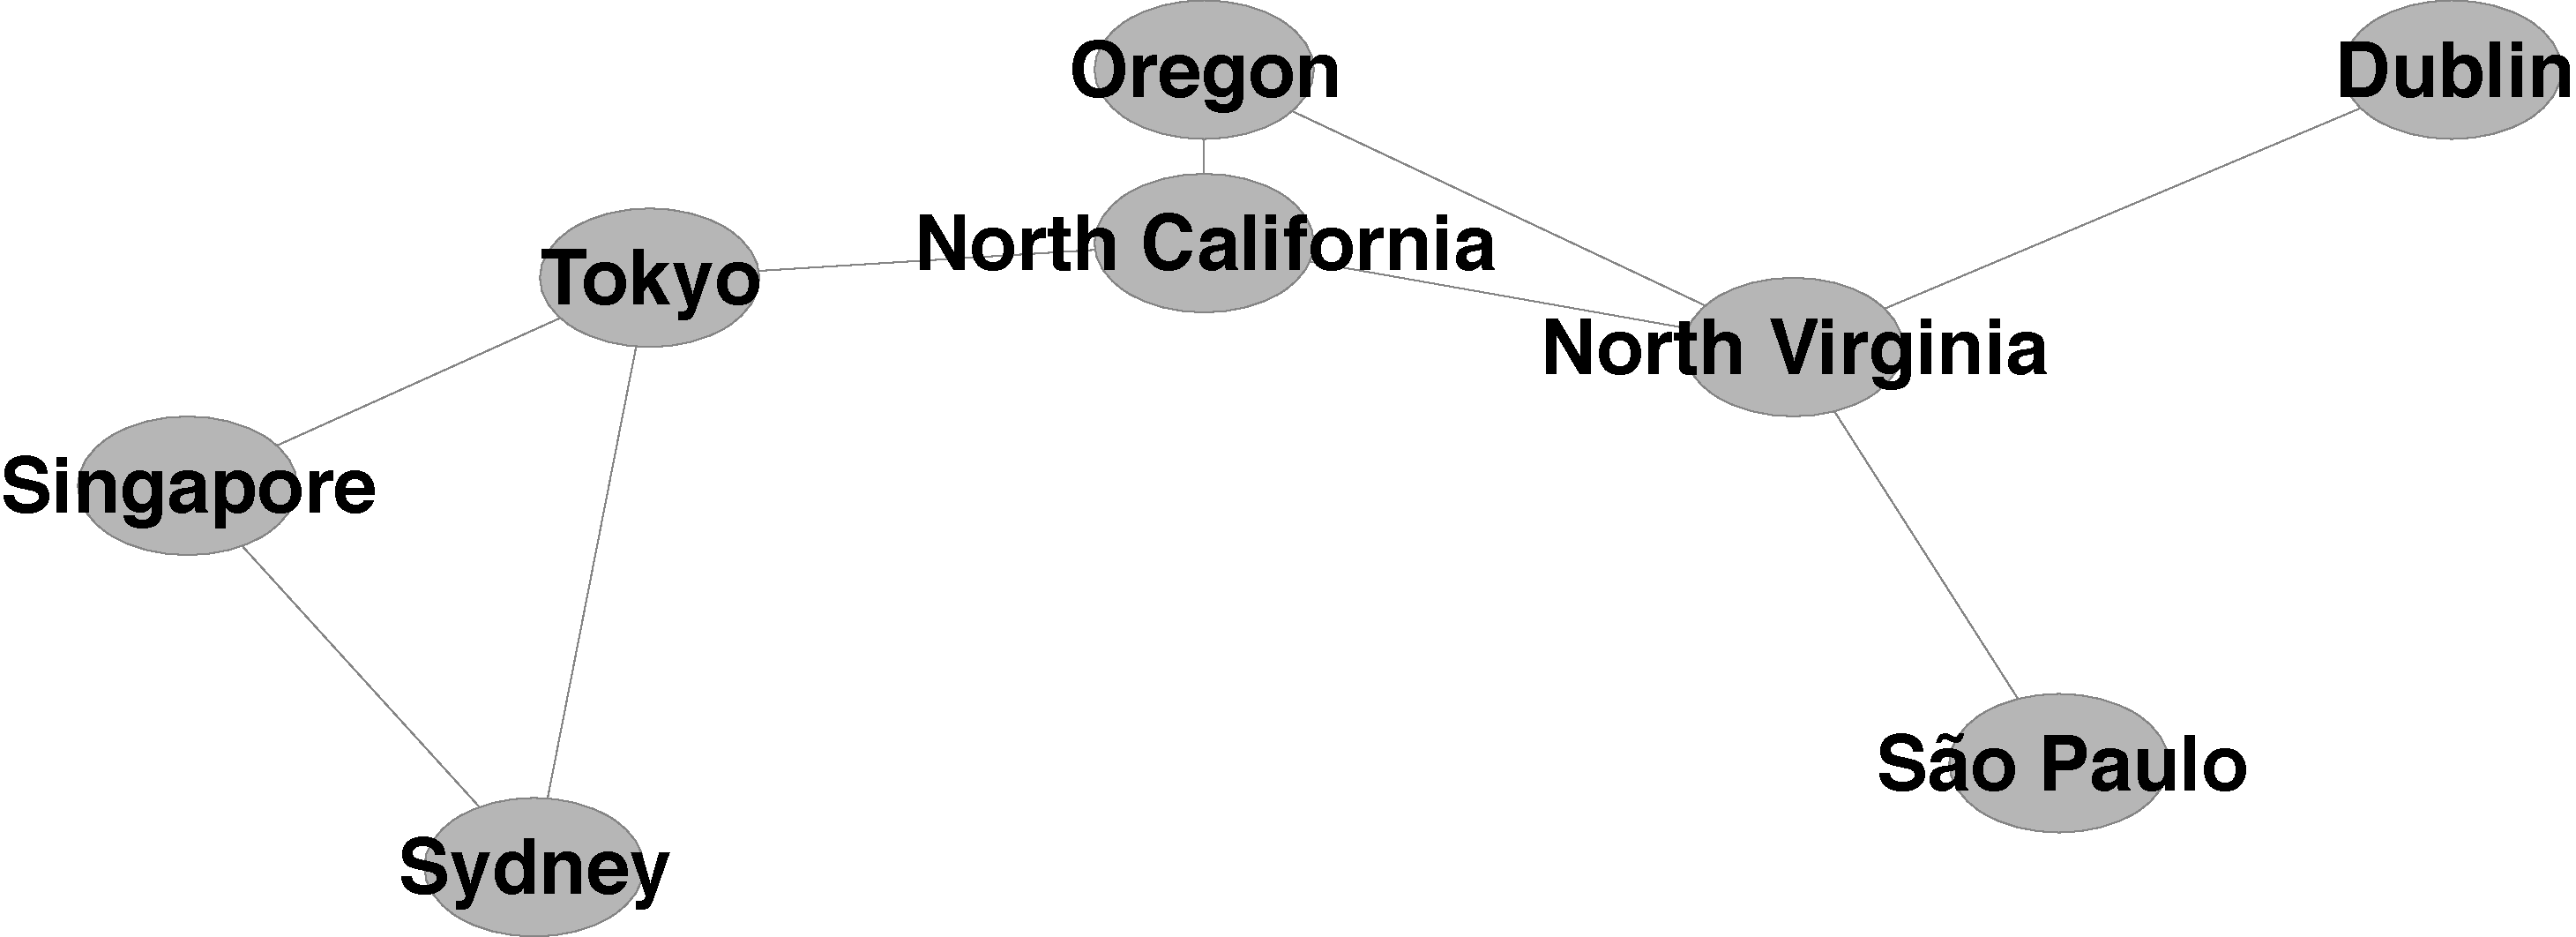
\includegraphics[width=.7\linewidth]{figures/loadbalancing}
  \caption{Small load balancing network \citep{garant2015accelerating}}
  \label{fig:loadbalancing}
 \end{center}
\end{figure}

\section{Methods} \label{sec:methods}
Several questions arise when designing a solution for this problem: How to identify groups in which information sharing is possible? What information should be transferred between agents in those groups? How can convergence in distributed and concurrent settings be guaranteed? This section provides a high level overview of the author’s conceptual framework and associates their scheme with our implementation of the model.  We highlight several design decisions and attempt to provide insights in difficulties and non-trivialities that pop up in the implementation process.

\subsubsection{Supervisory Architecture}
The authors propose a model of supervisor and subordinate agents. The subordinates can be seen as the domain specific workers of the system that aim to optimize a joint, domain-specific problem (e.g. load balancing distribution to minimise total service time). Supervisors keep track of subordinate groups and aim to accelerate the learning process using high level feature traits, collected from the subordinates.

The process starts by creating \textit{subordinate groups} (Figure \ref{fig:subordinate}) consisting of supervisors and subordinates. These groups remain fixed over the entire learning process. After groups are formed, supervisors periodically search for \textit{contextual compatible} subordinates in their subordinate group to compose experience \textit{sharing groups}. In these groups, subordinates are able to share learned experiences with any other member from the sharing group. Experience sharing between subordinates from different supervisors is not allowed. The contextual compatibility is determined by a distance measure over context features between two agents. These context features can depend on factors like metric-defined interactions within a certain group of agents, or aggregate effects over group interactions (e.g. amount of sent messages between agents over a time period).
\begin{figure}[H]
 \begin{center}
  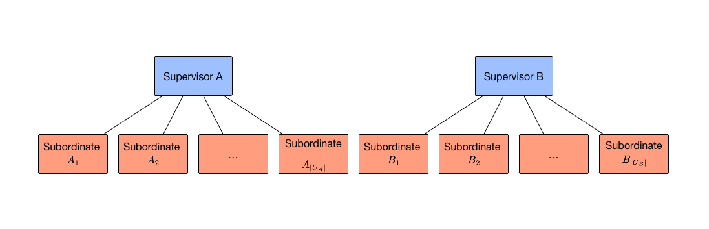
\includegraphics[width=\linewidth]{figures/subordinates}
  \caption{Supervisor hierarchy \citep{garant2015accelerating}}
  \label{fig:subordinate}
 \end{center}
\end{figure}

In order to keep the shared experiences concise, time-windows of $t$ timesteps are defined to characterize policy, reward and transition changes. Considering that decisions are framed as a Markov Decision Process (MDPs), experiences for one time window $[t_{0}, t_{e}]$ can be represented as a vector of tuples with $s_i, a_i, r_i$ and $s'_i$ corresponding to current state, action, reward and next state of the subordinate as depicted in figure \ref{fig:tuples}. To be even more concise, another possibility would be to merge experiences within a given time window. This is disregarded due to increased complexity and information loss risks when states are not visited uniformly.
\vspace{\baselineskip}
\begin{align*}
 \biggl<
  & (s_{i_{t_0}},a_{i_{t_0}},r_{i_{t_0}},s'_{i_{t_0}}), \\
  & (s_{i_{t_1}},a_{i_{t_1}},r_{i_{t_1}},s'_{i_{t_0}}), \\
  & \hdots                                              \\
  & (s_{i_{t_e}},a_{i_{t_e}},r_{i_{t_e}},s'_{i_{t_0}})
 \biggr>
\end{align*}
\begingroup\vspace*{-\baselineskip}
\captionof{figure}{Vector of experience tuples} \label{fig:tuples}
\vspace*{\baselineskip}\endgroup

In a real word setting, experiences could be compressed using linear regression, fitted to variable sets in the window. This is especially effective when agents infrequently change state. These \textit{compressed experiences} can be shared between subordinates using a supervisory agent as proxy. This allows the supervisor to derive context features from reported experiences and share it with subordinates that desire so. Though useful to save network bandwidth in a practical sense, from a theoretical point of view, compression does not change the functionality of the system, and was omitted in our implementation since it only adds complexity. We chose to send raw, uncompressed experiences in order to update subordinates. The diagram below gives an overview of the model.
\begin{figure}[H]
 \begin{center}
  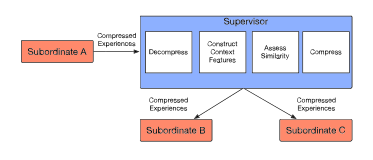
\includegraphics[width=\linewidth]{figures/diagram}
  \caption{Supervisory structure \citep{garant2015accelerating}}
  \label{fig:diagram}
 \end{center}
\end{figure}

To conclude the author’s theoretical framework we discuss how context features are constructed from the experiences that are passed along. We note that features like experience imbalance, policy divergence, unobservable state features and disjoint state visitations are attention points to take into account during context feature construction. More information on these concepts can be found in the paper. Since the context feature construction is domain-dependent, the authors only provide a general approach for doing so. The following paragraphs will explain our approach dealing with the proposed problem, but also ambiguities and missing information.

\subsubsection{Random Graph, Supervisory Topology, Task Allocation}
For each trial, a random network is generated for the given size and branching factor parameters. The supervisor topology is then imposed randomly on this network, differing from the original where the subordinate group of a supervisor is a highly connected cluster.  Since the supervisor assignment is random, no assumptions can be made about the connectivity of other agents in the subordinate group. In addition, tasks are randomly allocated with random service time. The goal of utilizing so much randomness in the construction of the simulations is to minimize design bias in the network and preclude any cross-domain assumptions that might creep in, especially in supervisor assignment.

\subsubsection{Worker Q-Learning with Softmax and Experience Integration}
Workers in the network improve their performance using a basic Q-learning algorithm with $\gamma = 0.1$ and a \textit{softmax} decision policy with $\tau = 0.1$.  Integrating experiences from other agents is done in a naive fashion, extracting the reward and neighbor index from the experience to update its corresponding Q-values for each shared experience.

\subsubsection{Distance Function}
The distance functions for each type of context feature follow a similar pattern that allows for proper interaction with the Boltzmann distribution used in the sharing selection algorithm.
\[D^C(C_1, C_2) = \lceil 10e^{-| C_1 - C_2 |} \rceil / 10\]

The quantized inverse exponential absolute difference produces discrete values that are near 1 when the distance is near 0 and and near zero when the distance grows large. This allows the Boltzmann distribution to correctly weight small context feature distances with higher probabilities.

\subsubsection{Context Feature Construction}
Although the paper states that context feature construction is a transformation of an agent’s experiences for a given window into a vector or context features, it is only possible to create the context features only from the experiences of an agent by encapsulating all of the information relevant to the context features in the state of the agent. This sounds trivial, but in this case requires recording the local state (i.e. load, environment task allocation rate, and agent task allocation rate) of each of its neighbors into its own state. Instead of encapsulating all of this data in this extended state, in our implementation the supervisor queries the agent and its neighbors for the information it requires and creates the context features from those responses.  These two methods are equivalent because the exact same information is gathered from querying as extracting from state. This allows us to have a simpler state representation.

\section{Results and Discussion}
To present our results, we use the same methodology as the original paper to facilitate comparison. The primary measure of performance is the \textit{Area Under the Learning Curve} (AUC). It is computed by taking the difference between the originally assigned service time of each task and the actual time needed by the network to solve it. The mean of this difference in service time per time step is then smoothed using an exponential moving average with a smoothing factor $\alpha=2/(span+1)$, where \textit{span} is set to the time period for which the simulation was run (i.e. $10,000$). The minimum mean value is then subtracted from each remaining value to "lower" the curve onto the x-axis. Taking the area under this curve results into the AUC measure. This measure reflects the performance of a parameterization of the algorithm, as we want the difference in assigned and consumed service time to be as small as possible over as long a time span as possible, which is precisely what the AUC provides.

Figure \ref{fig:areas} gives an example of the baseline architecture compared to the one supervisory configuration. To facilitate reproduction of our results, we provide, for each figure, the exact parameterization used to generate it. We will use, where applicable, $S$ for the number of supervisors, $K$ for the size of the learning window, and $N$ for the size of the network. Unless specified otherwise, all simulations use a \textit{maximum branching factor} of $10$ and a \textit{maximum service time} of $50$ and the results are the average over 30 trials. When we speak of the \textit{baseline configuration} the following parameters were used: $S=0,K=25,N=100$.
\begin{figure}[H]
 \begin{center}
  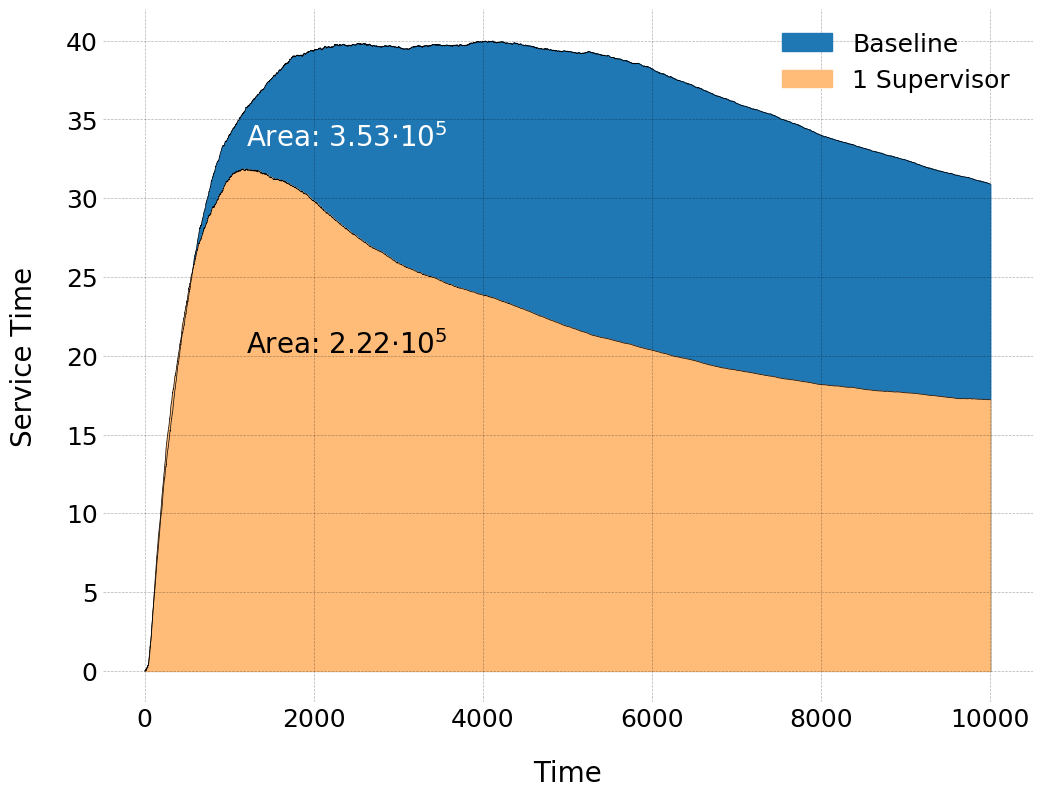
\includegraphics[width=\linewidth]{figures/figure5_light}
  \caption{Task Allocation Performance Evaluation\\Parameters: $K=25,N=100$}
  \label{fig:areas}
 \end{center}
\end{figure}

Clearly, the one supervisory configuration performs much better than the baseline configuration. In the beginning, when the network has not yet learned to distribute the load, the average service time rises quickly. Around 1000 time steps however, the supervisor has identified sharing groups and optimizes the learning process of the subordinates, resulting in fast convergence to a better task distribution. The agents in the baseline configuration also learn to distribute tasks, but do so at a much slower pace and with less success. Compared to the figure 5 of the original paper, the results qualitatively comparable, but not identical. The rate and difficulty of the tasks generated by the environment seem to be higher, as the maxima for both the baseline and one supervisor learning curve are stronger. 

As noted in the original paper, the parameters of the network had to be tweaked to yield significant results.  If the network topology and task allocation was too easy or too difficult, no appreciable difference is seen when using the supervisory framework.  Therefore, we and the original authors had to tweak parameters until we found that "goldilocks zone".  Since the original authors gave no detailed guidance in constructing the network or allocating tasks, it makes sense that our results are not exactly the same, since our parametrizations were undoubtedly different, though we still see the same general trend.

To see the effect of changing the parameters of the model, we will now take a look at a performance evaluation for different learning window sizes $K$. The AUC is not compared directly, but in comparison to the baseline architecture (for which changes in the learning window have no effect). Figure \ref{fig:windows} below depicts the results.
\begin{figure}[H]
 \begin{center}
  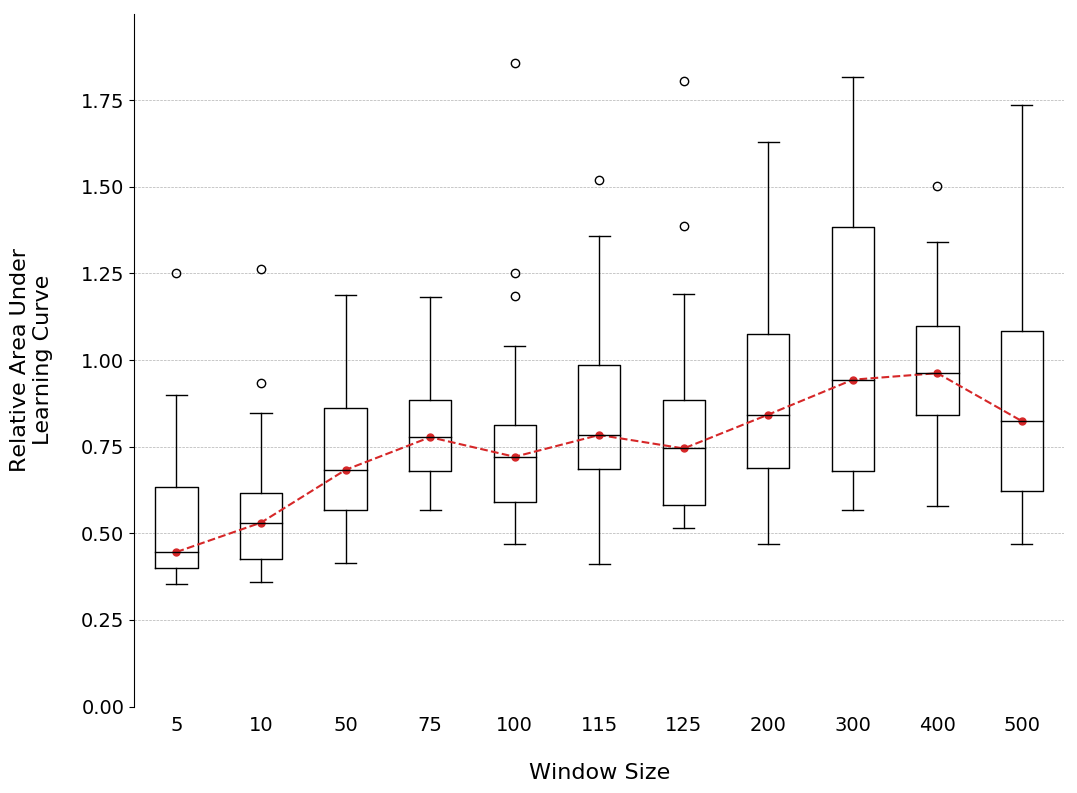
\includegraphics[width=\linewidth]{figures/figure4_extended}
  \caption{Effect of varying winow size K\\Parameters: $S=1/0,N=100$}
  \label{fig:windows}
 \end{center}
\end{figure}

Again, our results compare well to those seen in the paper. A rise in $K$ is generally positively correlated with a rise in relative AUC. There are occasional outliers, just like in the paper, which could be due to small sample size. The biggest difference is, that even for $K=500$ the performance of the one supervisory configuration still outperforms the baseline. As described before, this is most likely due to differing environment settings from the original.

In figure \ref{fig:sups} we explore the effect on the learning behavior when using a greater number of supervisors. The one supervisor scenario is a best case assumption, where sharing groups can be formed between the best suited candidates from the entire population of agents. With a rising number of supervisors the probability to identify contextually similar agents decreases due to smaller subordinate groups, resulting in a loss of performance. This effect can be observed in both our results and those from \citeauthor{garant2015accelerating}
\begin{figure}[H]
 \begin{center}
  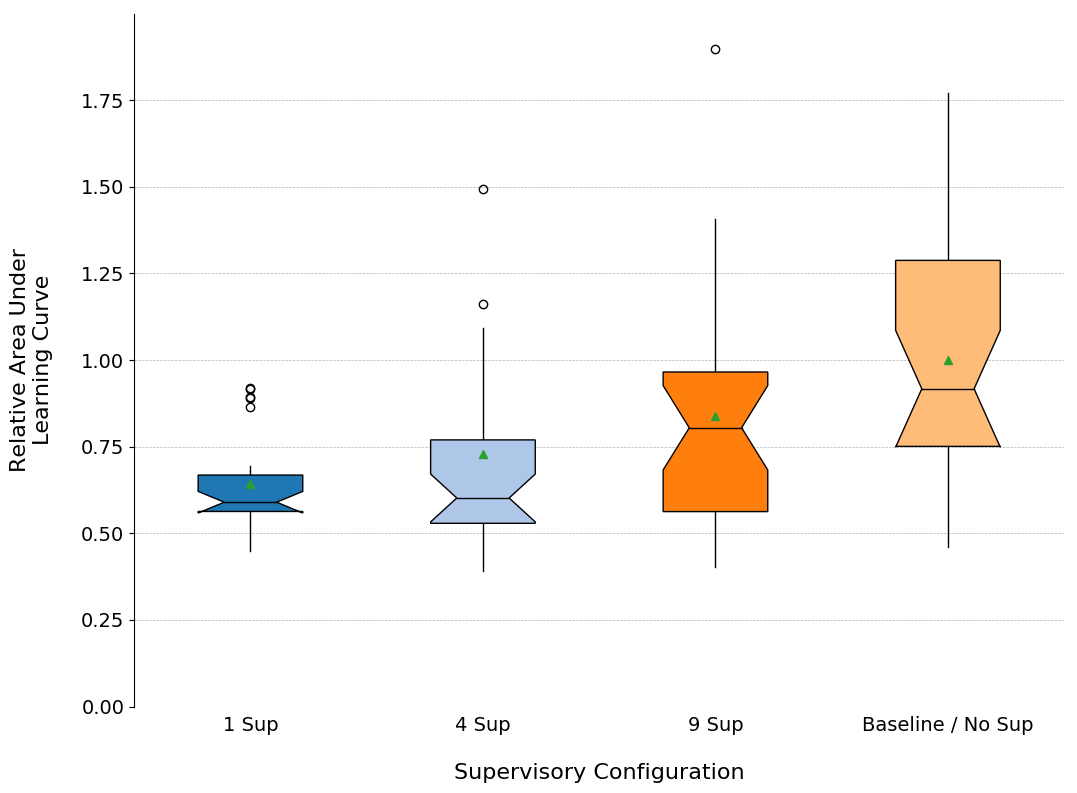
\includegraphics[width=\linewidth]{figures/figure7}
  \caption{Relative Performance by Supervisory Config.\\Parameters: $K=25,N=100$}
  \label{fig:sups}
 \end{center}
\end{figure}

While the variance of the results increases with a growing number of supervisors, consistent with the reference, it does so more rapidly in our work. Additionally the variance of the baseline configuration is much higher, possibly due to a different approach in computing the \textit{relative} AUC for which there is unfortunately no information provided in the original work. Our approach takes the average over all 30 trials of the baseline configuration to reference against. To highlight the trend towards the baseline performance when adding supervisors, we also display the mean value for all trials represented as small green triangles.
\begin{figure}[H]
 \begin{center}
  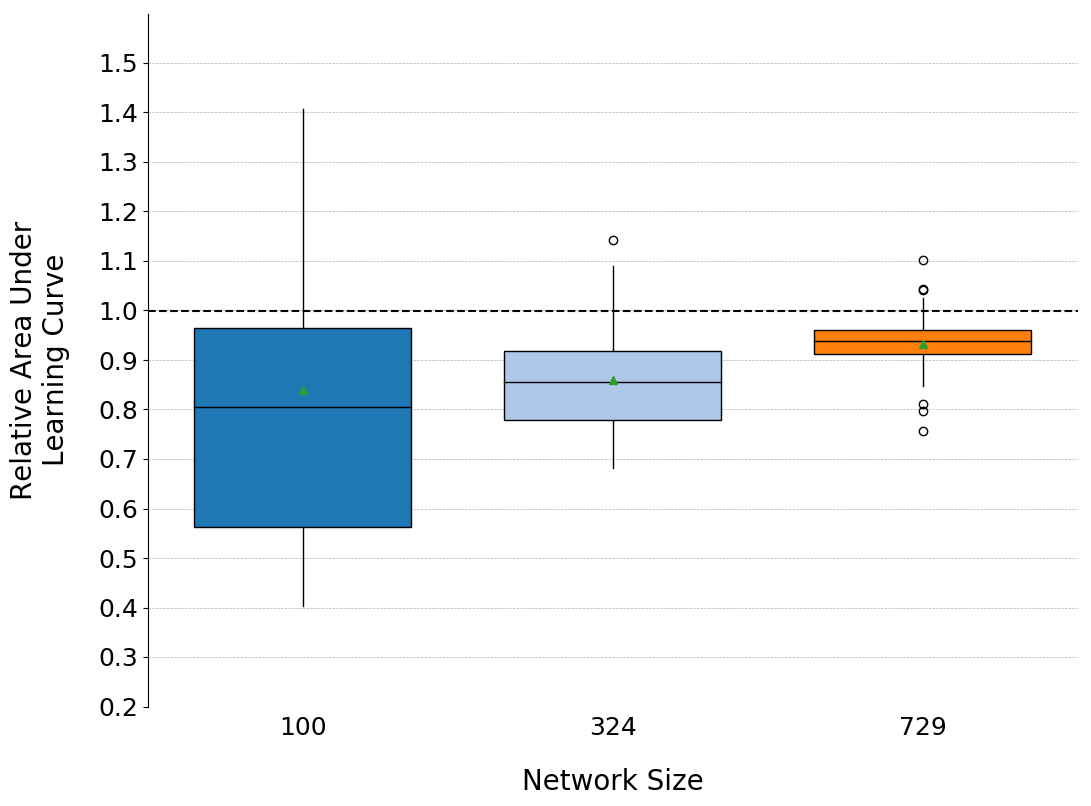
\includegraphics[width=\linewidth]{figures/figure8}
  \caption{Relative Performance as network size is varied\\Parameters: $S=1/0,K=25$}
  \label{fig:sizes}
 \end{center}
\end{figure}

The last parameter influence we want to explore is the network size. Figure \ref{fig:sizes} shows the relative performance of three different sizes against their respective baselines. It has to be noted, that individual baseline data had to be generated for each network size, as this is the first parameter affecting its performance. Here we see the first real divergence from the results seen in the paper. While in the original work performance increases with growing network size--explained by the increase in sharing opportunities per supervisor (see also Figure \ref{fig:sups})--it drops in our approach. Another notable difference is the drastic decrease in variance when growing the network while this cannot be observed in the reference work.

This difference from the original paper is most likely due to recurring "goldilocks zone" problem.  The parameters were tuned to fall within this zone--where the network topology and task allocation are neither too easy nor too difficult--for the $N=100$ network size.  Adding more nodes to the network makes the problem easier, because there are more nodes to spread the task processing around.  That is why we see less of an advantage for larger networks: when a problem is too easy, sharing experiences has only a marginal effect because there is less room for improvement.  We attempted to scale the relevant parameters to make the load-balancing problem the same difficulty for the larger networks as the $N=100$ network, but there are no metrics to precisely determine the difficulty of the load-balancing problem provided by the original paper, and so approximating equivalent problem difficulties between different network sizes comes down to guesswork, and was therefore omitted.

\section{Conclusion}
Though the original paper presents a compelling, and at-the-surface general, approach to sharing experiences between agents, during the implementation of their methods, we found problems, inconsistencies, and ambiguities that we take issue with.  Described here are two of the most problematic:
\subsubsection{Criticism: Context Feature Construction}
The choice of context features heavily influences the representation of the state of an agent.  For example here, an agent records information in its state that one would intuitively include, like the loads and rates of each of its neighbors.  In multi-agent reinforcement learning, agents generally want to make decisions based solely on information gained from reward signals, in this case obtained from neighbors.  It seems odd then to need to record the internal state of those neighbors for the context features to be created solely from experiences.  If you choose a more intuitive representation of state--i.e. information completely local to the agent--then creating the context features outlined in the paper is impossible. That is why we employed the querying implementation methodology, because information required to create the defined context features could not be recovered from experiences alone without being extremely “generous” in what counts as the state of an agent.

The problem stems from the fact that supervisor has no knowledge of the problem domain a priori, and therefore must extract all information from experiences. To see why it is impossible to extract context features from experiences alone, consider the following intuitive representation of an experience for the load-balancing problem, over a time window of size K:
$$ s = (load, rate_e, rate_a); a = Process | Forward(i) $$
The supervisor can recover the neighbors of the agent by looking at where the agent has forwarded to this window.  That might not be all, or any, of its neighbors so it only recovers a subset of those neighbors.

If the supervisor is allowed to look at other experiences of other agents in its memory--which the paper does not explicitly allow, but seems reasonable--then we can recover the relevant information from the experiences of the agents that are neighbors of the given agent, but only if those neighbors are in the supervisor’s memory.

Therefore, to get all of the information necessary to accurately calculate the context features for a given agent, that agent would have had to forward to all of its neighbors at least once in the window and those neighbors would also have had to be part of the same subordinate group.  Except for the single supervisor case, it is impossible for a subordinate group to completely surround a network cluster, meaning that not all neighbors will be in the supervisor's memory.

Since this intuitive representation is untenable, we have to choose between using a bloated, unintuitive, and pragmatically inviable representation of state, or just querying the agents for the information we require.  We chose the latter, eventhough it breaks the definition of context feature construction as a transformation from a single window of experiences to a vector of context features.  We believe the original authors did so as well.

\subsubsection{Criticism: The Goldilocks Zone}
As noted multiple times earlier, most of the results of this and the original paper are predicated upon the network topology and task allocation problem difficulty.  If the problem is too easy, there is not much room for improvement, and we see decreased or negligible gains from sharing experiences.  If the problem is too difficult, sharing experiences has no effect because even behaving optimally, the network cannot keep up.  Therefore, parameters have to be tuned so that we're in the "goldilocks zone" where sharing experiences has a significant effect.  In the end, the results of the original paper should have given a larger caveat that they tuned their network to a difficulty that makes their results significant, or ideally, present a metric to explicitly define this "goldilocks zone", so we know when sharing experiences will have a significant effect beforehand.

\subsubsection{Summary}
This paper reviewed a method to accelerate learning in MAS, proposed by Garant et al. (2015). By means of a personal implementation, we examined theoretical and empirical analysis of the authors. This allowed us to reason and comment on design decisions, metrics, optimizations and ambiguities that followed from the work. After providing an introduction and methodology background, we highlighted implementation details and concluded the paper with our obtained results and corresponding discussion. Overall, we observed comparable results with slight variance but noted that these results were very sensitive to MAS and architecture settings.

\subsubsection{Outlook}
In the future, there are a few interesting avenues of inquiry regarding context features and experience sharing:

As noted earlier, a defined metric definition of the "goldilocks zone" would be useful in determining what problem instances will benefit from the supervisory architecture.  Especially if altering the parameters of the problem is difficult or impossible, it would be useful to determine beforehand if sharing experiences will have a significant effect.  Having a defined metric for this would determine where the supervisory structure is applicable.

In relation to context features, an analysis of the quality vs. quantity tradeoff would be useful.  For instance, suppose that there is a context feature that produces great gains, but is expensive to compute.  There may instead be other context features that are simple to compute, but have limited effect on improvement.  It would be interesting to investigate if many low-quality context features used in conjunction provide similar improvement as a few high-quality context features, and therefore save on computational complexity.

Another avenue may be to extend reinforcement learning to the supervisor.  Since currently, supervisors only perform computation and communication, there is no learning or improvement occurring within a supervisor.  If the subordinate could respond to the supervisor with a reward signal when it receives experiences, the supervisor may be able to use it to learn more about what context features are effective, or which subordinates respond well to shared experiences, allowing the supervisor to improve its context feature construction and sharing group selection.

\\\todo{Make sure all questions given below are answered}
\begin{enumerate}
 \item Does the introduction explain clearly the content of the paper - Maybe not?
 \item whether there is sufficient background information to understand the relevance of the work - Yes!
 \item whether the methods are clearly explained (can the results be reproduced?) - Yes!
 \item whether the results answer the questions asked in the paper. \todo{Identify questions}
 \item whether all questions are answered - Which ones??
 \item whether the conclusion is sufficient - We'll see.
 \item and whether the overall style is ok and - Oh yes!
 \item whether you believe things are missing in the discussion. - Nope.
 \item etc. - Yes.
 \item 3 positive points concerning the work, clearly specifying why you think they are well-done or interesting
 \item 3 negative points, which may include missing/unclear explanations or suggestions for improvement
 \item at least 3 clear and relevant questions on the content or the methods used which can be asked (next to other questions).
\end{enumerate}

\footnotesize
\bibliographystyle{apalike}
\bibliography{bibliography}

\end{document}
